% ****** Start of file apssamp.tex ******
%
%   This file is part of the APS files in the REVTeX 4.2 distribution.
%   Version 4.2a of REVTeX, December 2014
%
%   Copyright (c) 2014 The American Physical Society.
%
%   See the REVTeX 4 README file for restrictions and more information.
%
% TeX'ing this file requires that you have AMS-LaTeX 2.0 installed
% as well as the rest of the prerequisites for REVTeX 4.2
%
% See the REVTeX 4 README file
% It also requires running BibTeX. The commands are as follows:
%
%  1)  latex apssamp.tex
%  2)  bibtex apssamp
%  3)  latex apssamp.tex
%  4)  latex apssamp.tex
%
\documentclass[%
 reprint,
%superscriptaddress,
%groupedaddress,
%unsortedaddress,
%runinaddress,
%frontmatterverbose, 
%preprint,
%preprintnumbers,
%nofootinbib,
%nobibnotes,
%bibnotes,
 amsmath,amssymb,
 aps,
%pra,
%prb,
%rmp,
%prstab,
%prstper,
%floatfix,
]{revtex4-2}
\usepackage{kotex}
\usepackage{graphicx}% Include figure files
\usepackage{dcolumn}% Align table columns on decimal point
\usepackage{bm}% bold math
\usepackage{tikz}
\usetikzlibrary{arrows}

% Nice captions.
\usepackage[hang,small,bf]{caption}
\setlength{\captionmargin}{25pt}

% New commands to keep things tidy.

%\usepackage{hyperref}% add hypertext capabilities
%\usepackage[mathlines]{lineno}% Enable numbering of text and display math
%\linenumbers\relax % Commence numbering lines

%\usepackage[showframe,%Uncomment any one of the following lines to test 
%%scale=0.7, marginratio={1:1, 2:3}, ignoreall,% default settings
%%text={7in,10in},centering,
%%margin=1.5in,
%%total={6.5in,8.75in}, top=1.2in, left=0.9in, includefoot,
%%height=10in,a5paper,hmargin={3cm,0.8in},
%]{geometry}

\def\rcurs{{\mbox{$\resizebox{.16in}{.08in}{
\includegraphics{ScriptR}}$}}}
\def\brcurs{{\mbox{$\resizebox{.16in}{.08in}{
\includegraphics{BoldR}}$}}}
\def\hrcurs{{\mbox{$\hat \brcurs$}}}

\begin{document}


\title{마이켈슨 간섭 실험 보고서}

\author{서울대학교 전기정보공학부 2018-12432 박정현}
 \email{alexist@snu.ac.kr}
\date{실험일 : 10/23/2023, 제출일: \today}% It is always \today, today,
             %  but any date may be explicitly specified

\begin{abstract}
본 실험에서는 마이켈슨 간섭계를 이용해 거리에 따른 보강, 상쇄 간섭을 측정하여 이를 통해 레이저의 파장을 측정하였다. 측정값은 약 $675.7nm$였으며 참값과 $4\%$의 오차를 가졌다. 실험의 오차 원인으로 낮은 데이터 수, 그리고 마이크로미터를 이용해 이동하는 거울이 레이저와 평행하지 않은 것으로 결론지었다. 이를 해결하기 위해 거울의 각도를 변화하며 측정하는 방법, 그리고 자동화된 극대, 극소 측정 방법을 제시하였다.
\end{abstract}

%\keywords{Suggested keywords}%Use showkeys class option if keyword
                              %display desired
\maketitle

%\tableofcontents

\section{\label{sec:level1}Introudction}
\subsection{\label{sec:level2}마이켈슨 간섭계}
마이켈슨 간섭계는 Fig.\ref{fig:Michelsonl}와 같다. 반은 거울을 이용해 일정 부분의 빛은 투과시키고 일정 부분의 빛은 반사시켜 스크린에 간섭무늬를 만든다. 본 실험에서 나타나는 간섭무늬는 원형 무늬에 해당한다. 이 때 마이크로미터를 조절하면 각 거울에 반사되는 빛의 광경로 차이를 변화시킬 수 있어 간섭무늬의 극대 극소 위치 또한 변화하게 된다. 거울의 위치를 $d$만큼 이동시킨 경우 총 광경로 차이는 $2d$만큼 차이가 나게 된다. 따라서 마이크로미터를 조절하며 $n$개의 극대, 극소 위치가 변화한 경우 아래의 식이 성립한다.[1]

\begin{figure}[h]
    \centering
    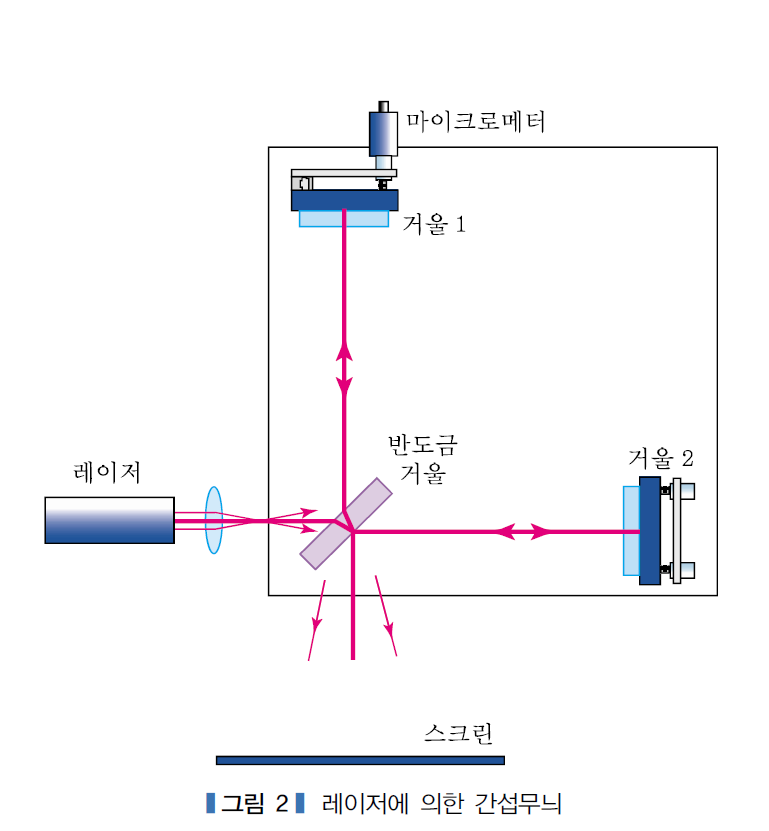
\includegraphics[width=0.8\linewidth]{Michelson.png}
    \caption{\label{fig:Michelsonl} 마이켈슨 간섭계}
\end{figure}

\begin{align}
	\frac{2}{\lambda}d &= n
\end{align}

\section{\label{sec:level1}Data \& Results}
각 거리에 따른 극대 극소 변화 값은 Fig.\ref{fig:data}와 같다. 이를 통해 계산된 빛의 파장값은 (\ref{eq:wave})와 같다. 주어진 레이저의 파장값 $650nm$와 약 $4\%$의 오차를 가진다.

\begin{figure}[h]
    \centering
    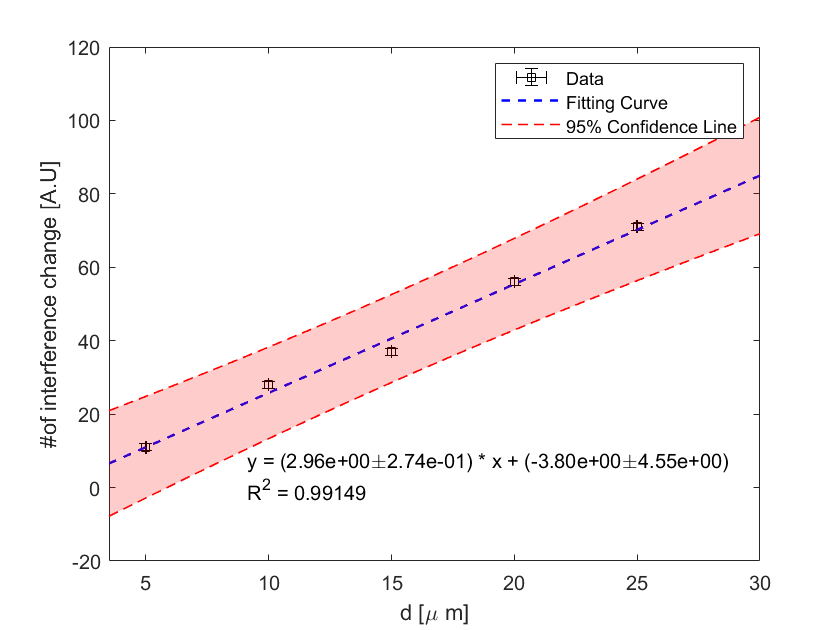
\includegraphics[width=0.95\linewidth]{data.png}
    \caption{\label{fig:data} 극대 극소 변화 측정 값}
\end{figure}

\begin{align}
	\lambda &= 675.7 \pm 31.3 nm \label{eq:wave}
\end{align}

\section{\label{sec:level1}Method}
붉은색 레이저를 킨 뒤 마이컬슨 간섭계에 조사한다. 이후에 레이저에 입사하는 볼록렌즈의 위치를 이동시켜 스크린에 원형 간섭문늬가 생기도록 한다. 이때 레이저, 볼록렌즈로 주어진 두개의 자유도를 활용하며 레이저는 어느정도 스크린에 레이저가 나타나도록 한 뒤 볼록렌즈를 이용해 미세하게 조정한다. 이후에는 스크린에 나타나는 극대, 극소를 마이크로미터를 이동시키며 카메라를 이용해 촬영한 후 몇개의 극대가 이동했는지 측정한다. 이러한 실험을 $5, 10, 15, 20, 25\mu m$의 거리를 이동시키며 반복한다.

\section{\label{sec:level1}Conclusion \& Discussion}
측정된 레이저의 파장값은 매우 낮은 오차값과 재현도를 가진다. 해당 실험에서 주어진 오차는 마이크로미터를 이용해 거울을 움직일 때 거울이 정확하게 레이저와 평행하게 이동하지 않아 발생한 오차로 결론지었다. 주어진 실험에서 거울이 움직이는 방향벡터와 레이저의 방향벡터 사이의 각도를 $\theta$로 두는 경우 식은 (\ref{eq:fixed})와 같아진다. 따라서 측정되는 파장값은 (\ref{eq:fixedwave})와 같아져 더 높은 파장값이 측정된다. 주어진 식을 이용해 기울어진 각도를 계산하면 약 $16^{o}$에 해당한다. 이를 해결하기 위해 마이크로미터를 이용해 거리에 따른 간섭무늬를 측정한뒤 이를 마이크로미터의 각도를 바꿔가며 반복해 각 경우에 따른 파장값을 측정해 해당 값 중 최소값을 파장값으로 측정하는 방법을 이용할 수 있을 것이다.

\begin{align}
	\frac{2}{\lambda}d\cos\theta &= n\\
	&\simeq \frac{2}{\lambda}d\left(1-\frac{1}{2}\theta^{2}\right)\label{eq:fixed}
\end{align}

\begin{align}
	\lambda_{meas} &\simeq \lambda \left(1+\frac{1}{2}\theta^{2}\right)\label{eq:fixedwave}
\end{align}

데이터의 수가 늘어나는 경우 통계적으로 실험 측정값은 더 낮은 오차를 가진다. 하지만 주어진 실험에서 보강, 상쇄 간섭의 변화는 육안으로 측정하였으며 큰 수의 데이터에서는 이러한 방법에 한계가 존재한다. 이를 해결하기 위해 CCD카메라, 혹은 PMT를 이용해 데이터를 측정해 기록하고 컴퓨터를 이용해 극대 극소의 변화를 측정하는 방법이 있을 것이다.

\section{\label{sec:level1}Reference}

[1] Halliday, D., Resnick, R., \& Walker, J. (2013, August 5). \textit{Fundamentals of Physics}. Wiley.

\end{document}
%
% ****** End of file apssamp.tex ******
